Nach dem Verknüpfen der Bilder verbleiben neben den Defekten noch schmale horizontale Streifen (vgl. Abbildung \ref{img:minAndMaxLink} und \ref{img:diffImage}).
Wenn man die beiden Kamerabilder mit phasenverschobenen Streifenmustern übereinanderlegt, bilden sich Überlappungen der Streifen.
Diese können durch eine Reihe an Ungenauigkeiten im gesamten Prozess entstehen.
Zum besseren Verständnis muss auf die Differenzen zwischen dem aufgenommenen Kamerabild und der tatsächlichen Szene eingegangen werden.

\p
Das Kameraobjektiv hat bestimmte Einstellungsmöglichkeiten.
Aufgrund der festen\linebreak Brennweite des verwendeten Objektivs, wird der Einfluss der Brennweite nicht genauer betrachtet.
Die entscheidenden Einstellungen für diesen Prozess sind also der Fokus und die Blende.
Über die Fokussteuerung kann eine einzelne Tiefenebene im Bild scharf gestellt werden.
Da das Prüfobjekt und das Streifenmuster in unterschiedlichen Tiefenebenen liegen, führt das bereits dazu, dass im Kamerabild nicht beides gleichzeitig fokussiert werden kann.
Der Fokus liegt zur Prüfung auf der Oberfläche des Objekts.
Dadurch wird das Streifenmuster unter Umständen unschärfer, wodurch die Breiten der hellen und dunklen Streifen verändert werden.
Die zweite Einstellungsmöglichkeit ist die Blende.
Öffnet man diese weiter, lässt man mehr Licht in den Kamerasensor.
Durch mehr einfallendes Licht vergrößern sich die Breiten der hellen Streifen im Bild. 
Oberflächendefekte des Prüfobjekts werden gleichzeitig besser sichtbar.
Die Belichtung lässt sich auch über eine Nachbearbeitung verstärken.
Durch diese Beeinflussungen der Streifenbreiten müssen die Breiten der hellen und dunklen Streifen unter Berücksichtigung des Kamerabildes angepasst werden.
Beispielsweise sind die vertikalen Streifenbreiten der erzeugten Muster aus den Abbildungen \ref{img:imageToLink} - \ref{img:diffImage}, fünf Pixel für die hellen und neun Pixel für die dunklen Streifen.

\begin{figure}[H]
	\centering
	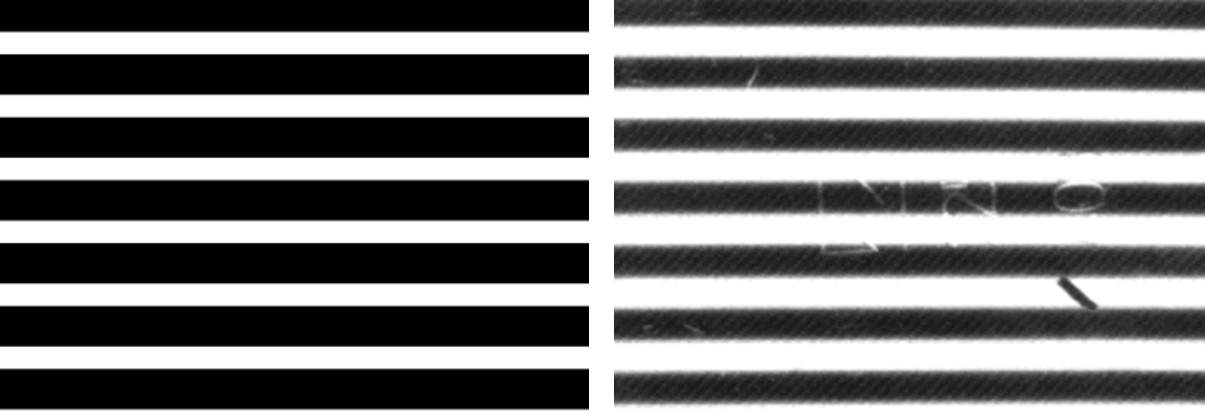
\includegraphics[width=\textwidth]{03_sichtpruefungDurchLichtreflexionen/optimierungen/figures/differenceCameraPattern}
	\caption[Unterschied zwischen Muster und Kameraaufnahme]{Unterschied zwischen Muster und Kameraaufnahme. Links erzeugtes Muster, Rechts Kameraaufnahme}
	\label{img:differenceCamPat}
\end{figure}

\noindent
Es kommt dazu, dass die hellen und dunklen Streifen im Kamerabild unter Umständen nicht exakt gleich breit sein können, da die Anpassung der Breiten der Streifen lediglich auf pixelgenauer Ebene durchgeführt werden kann.
Außerdem gibt es auch bei der Phase der Streifenmuster die Beschränkung, dass die maximale Genauigkeit der Verschiebung auch ein Pixel beträgt.
Das bedeutet, dass die Streifen selbst bei exakt gleicher Breite unter dem Kamerabild nicht genau versetzt voneinander liegen.
Es kommt hinzu, dass diese Genauigkeit sich auf den projizierenden Bildschirm bezieht.
Also ist der Phasenwinkel im Kamerabild durch die Messung auch mit Fehlern behaftet, weshalb sich die Fehler akkumulieren.

\p
Da die Kameraeinstellungen auf die Prüfstation und Prüfbedingungen angepasst werden müssen, sind die Mög\-lich\-kei\-ten zur Eliminierung der Streifen im Vorhinein begrenzt.
Die Nachbearbeitung kann über verschiedene Ansätze erfolgen.
Aufgrund der Periodizität und der festen Ausbreitungsrichtung der Streifen bietet es sich an, die Fourier-Analyse anzuwenden.
Man untersucht die Frequenzkomponenten der Streifen und filtert speziell diese aus dem Bild heraus, um sie zu entfernen.
Diese Methode kann allerdings nicht die fehlende Information an den dunklen Streifen wiederherstellen, sondern lediglich eine Bildverbesserung durchführen.
Eine andere Mög\-lich\-keit ist das Hinzuziehen von weiteren Bildern.
Da an den Stellen der horizontalen Streifen die Information fehlt, kann man wie auch schon zuvor zusätzliche Muster zur Hand nehmen, um die Information aufzufüllen.
Man zieht zwei weitere Muster hinzu, deren Überlappungen genau in den Zwischenräumen des verknüpften Bildes sind. 
Daraus kann man die Informationen vereinen und eliminiert die horizontalen Streifen.
Für dieses Verfahren sind damit vier Streifenmuster nötig, die je eine versetzte Phase zueinander haben.
Aus den vier aufgenommenen Bildern verknüpft man je zwei Bilder, die eine Phasendifferenz von $ \pi $ zueinander haben, mit der betragsmäßigen Differenz.
Die zwei resultierenden Bilder haben zueinander versetzte Streifen, die aus den Überlappungen entstehen.
Zum Schluss kann man die beiden Bilder so verknüpfen, dass man stets den Bildpunkt mit dem höheren Helligkeitswert nimmt.
Das entspricht der Maximierung.
Analog kann man auch die horizontalen Streifen aus Abbildung \ref{img:minAndMaxLink} eliminieren, in welcher die Typen von Fehlstellen isoliert voneinander betrachtet wurden.
In Abbildung \ref{img:imageTree} werden die einzelnen Schritte dieses Verfahrens veranschaulicht.

\begin{figure}[H]
	\centering
	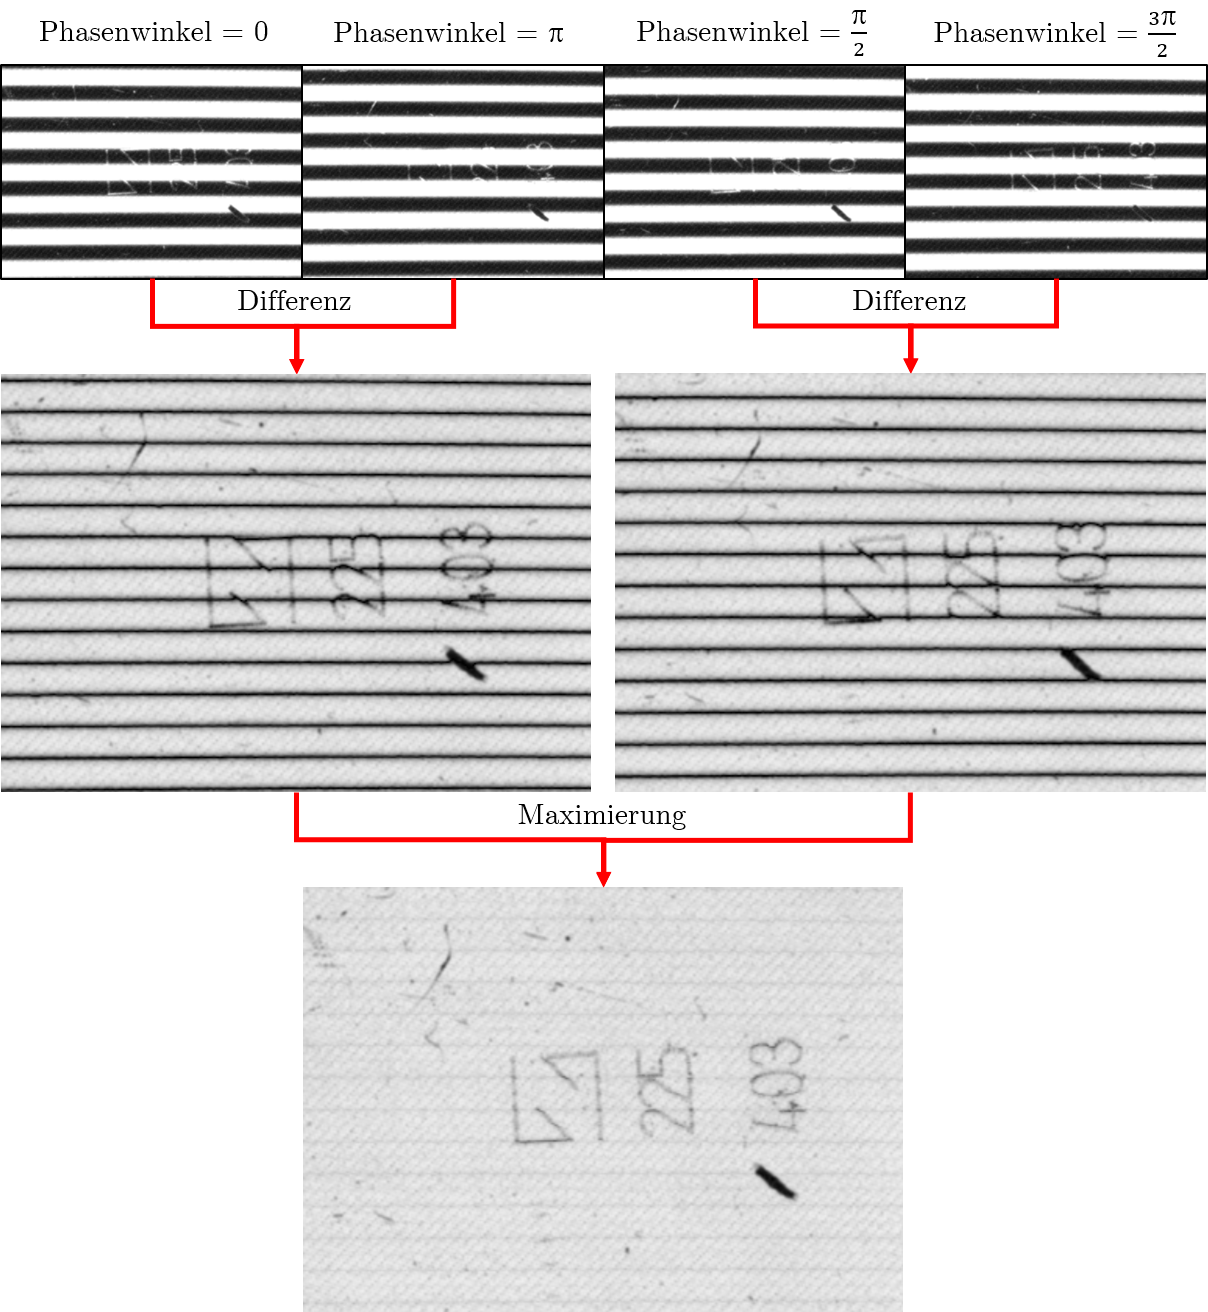
\includegraphics[width=\textwidth]{03_sichtpruefungDurchLichtreflexionen/optimierungen/figures/imageTree}
	\caption[Prozess der Hervorhebung von Oberflächendefekten]{Prozess zur Hervorhebung von Oberflächendefekten.}
	\label{img:imageTree}
\end{figure}

\noindent
Im praktischen Durchlauf verbleiben auch im letzten Bild noch sehr schwache horizontale Streifen.
Das liegt an den oben genannten Ungenauigkeiten im Prüfprozess, wodurch die vier Streifenmuster nicht exakt den angegebenen Phasenwinkel haben.
Deshalb kommt es dazu, dass die Überlappungen nicht exakt in den Zwischenräumen versetzt liegen und im Gesamtbild diese Struktur auftaucht.
Zur Bildverbesserung hat man nun noch die Möglichkeit, die zuvor erwähnte Fourier-Analyse anzuwenden.
Die noch verbliebenen Strukturen lassen sich im Amplitudenspektrum des Bildes durch die Ausbreitungsrichtung finden.
Da diese Strukturen nur noch sehr schwach im Bild vorhanden ist, sind die jeweiligen Frequenzkomponenten auch dementsprechend gering gewichtet (siehe Abbildung \ref{img:amplitudeSpectrum}).

\begin{figure}[H]
	\centering
	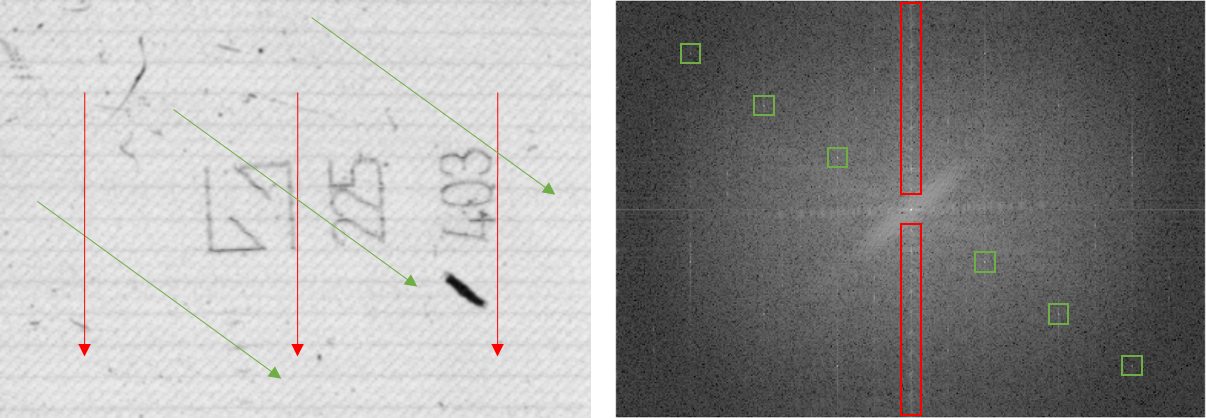
\includegraphics[width=\textwidth]{03_sichtpruefungDurchLichtreflexionen/optimierungen/figures/amplitudeSpectrum}
	\caption[Amplitudenspektrum des Gesamtbildes]{Amplitudenspektrum des Gesamtbildes. (mit Markierungen)}
	\label{img:amplitudeSpectrum}
\end{figure}

\noindent
In Rot ist im Bild die Ausbreitungsrichtung der ersten Struktur markiert, die entsprechenden Gewichte der Frequenzkomponenten sind in derselben Farbe im Amplitudenspektrum gezeichnet.
Analog sind in Grün die für die zweite Struktur relevante Ausbreitungsrichtung und Gewichte der Frequenzkomponenten markiert.
Filtert man im Amplitudenspektrum die markierten Bereiche heraus und wendet die Inverse Fourier-Transformation an, erhält man ein Bild, indem die beiden störenden Strukturen nicht mehr vorhanden sind.
Dies konnte derzeit nur durch ein geeignetes Online-Werkzeug \cite{fourierTool} ausprobiert werden.

\begin{figure}[H]
	\centering
	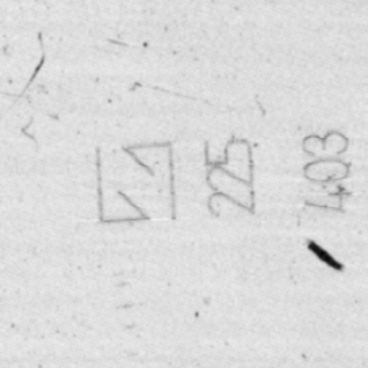
\includegraphics[width=0.4\textwidth]{03_sichtpruefungDurchLichtreflexionen/optimierungen/figures/frequencyFiltered}
	\caption[Bild mit angewandtem frequenzselektives Filter]{Angewandtes frequenzselektives Filter nach Abbildung \ref{img:amplitudeSpectrum}. Erstellt mit dem Online-Werkzeug \glqq Fourifier\grqq ~von © 2020 Ejectamenta.\cite{fourierTool}\footnotemark}
	\label{img:frequencyFiltered}
\end{figure}
\footnotetext{Anmerkungen: Das Bild musste aufgrund der Anforderungen des verwendeten Online-Werkzeugs zugeschnitten werden. Außerdem wurden die Frequenzkomponenten \glqq händisch\grqq ~entfernt, weshalb das Bild fehlerbehaftet ist. Das Bild konnte auch nicht auf Korrektheit geprüft werden und dient nur der Veranschaulichung. Die Nutzungsrechte unterliegen der Lizenz von © 2020 Ejectamenta. Für weitere Informationen zu Geschäfts- und Nutzungsbedingungen siehe: \url{https://ejectamenta.com/about/terms-of-service/}}

\noindent
Mit dem vorgestellten deflektometrischen Verfahren wurden Oberflächen\-de\-fekte wie z. B. Kratzer, Eingravierungen oder Partikel auf transparenten und spiegelnden Prüfobjekten sichtbar gemacht.
Das erzeugte Gesamtbild dieses Verfahrens kann nun durch anschließende Bildverarbeitung analysiert und geprüft werden.
In diesem konkreten Fall würden sich z. B. Kratzer detektieren oder die eingravierten Zeichen auslesen lassen.

\p
Geeignete Anpassungen der Parameter machen es möglich, diesen Prototyp für unterschiedliche Prüfobjekte, Aufbauten und Anforderungen anzuwenden.
Daraus ergibt sich das Ziel, eine allgemeine Lösung zu entwickeln, die mit möglichst wenig Aufwand für verschiedene Anwendungen genutzt werden kann.